\documentclass[journal]{IEEEtran}
%\usepackage[spanish]{babel}
\usepackage[utf8]{inputenc}
\usepackage{amsmath, amsthm, amsfonts}
\usepackage{graphicx}
\usepackage{cite}
\usepackage{listings}
\usepackage{tabularx}
\usepackage{multirow}
\usepackage{colortbl}
\renewcommand{\refname}{Referencias}
\usepackage{subfig}
\usepackage{booktabs}
\usepackage{cite}
\renewcommand{\citedash}{ -- } 

\renewcommand{\tablename}{\small{\textsc{Tabla}}}

\title{Análisis de Desempeño de Redes Inalámbricas de Sensores mediante Replicators Dynamics}

\author{\IEEEauthorblockN{~Jairo A. Caballero P. ~ ~ ~ ~ José L. Gutiérrez A.}\\
~\IEEEmembership{jacaballero@unal.edu.co} ~
~\IEEEmembership{...@unal.edu.co}\\
\IEEEauthorblockA{Maestría en Ingeniería Eléctrica\\
Departamento de Ingeniería Eléctrica y Electrónica\\
Universidad Nacional de Colombia.\\
Bogotá. Colombia.\\
}}

\renewcommand{\leftmark}{Optimización y Control en Sistemas Distribuidos en Red. J. Caballero, J. Gutierrez, Diciembre 10 de 2015} 
\begin{document}

\maketitle
\renewcommand{\abstractname}{Resumen}
\begin{abstract}
    En este artículo se presenta el desarrollo de un protocolo de comunicación ALOHA que....

\end{abstract}

\renewcommand{\IEEEkeywordsname}{Palabras claves}
\begin{IEEEkeywords}
 ALOHA, ALOHA ranurado, Balance de Energía, Desempeño, GETB, Poisson, , Population Games, Red Inalámbrica de Sensores,  Replicators Dynamics, Teoría de Juegos, WSN.

\end{IEEEkeywords}


\IEEEpeerreviewmaketitle

\section{Introducción}

\IEEEPARstart{H}{oy} en día .... AQUI SE AGREGA LA INTRODUCCIÓN

\section{Estado de Arte}

\subsection{Aplicación de teoría de juegos}



Para mejorar la calidad de los servicios en las redes de comunicaciones, se han realizado innovaciones en los protocolos de información así como en el mejoramiento de las tecnologías en este ámbito. Observando el aumento en las necesidades de los usuarios, se pretende usar usar nuevos modelos para mejorar la eficiencia de los recursos usados. Una de las técnicas más usadas es la \textit{"Teoría de Juegos"} la cual posee un amplio abanico de aplicaciones, especialmente en ingeniería, donde las acciones de cada componente tiene repercusión en los demás sistemas.


\begin{table*}[]
\centering
\caption{Teoría de Juegos aplicado a Redes Inalámbricas}
\label{Table_Game_Theory}
\begin{tabular}{|c|c|}
\hline
\textbf{COMPONENTE DEL JUEGO} & \textbf{ELEMENTO EN LA RED INALÁMBRICA}       \\ \hline
\textit{\textbf{Jugadores}}   & Nodos de la Red.                              \\ \hline
\textit{\textbf{Recursos}}    & Toda clase de recursos necesarios para que un nodo pueda comunicarse correctamente. (Espectro, 
\\
& Potencia, Ancho de Banda, etc).
\\ \hline
\textit{\textbf{Estrategias}} & Una decisión con respecto a una determinada acción del jugador, dependiendo del campo de aplicación
\\ 
& (de paquetes hacia adelante, nivel de potencia establecido, aceptar la nueva llamada, etc.). 
\\ \hline
\textit{\textbf{Pagos}}       & Estimado por funciones de utilidad, con base en los méritos de calidad de servicio (retardo, rendimiento, SNR, etc.).
\\ \hline
\end{tabular}
\end{table*}

Aún con lo anterior, se poseen algunos problemas al modelar este tipo de sistemas, algunos de los más importantes son:

\begin{itemize}
    \item \textit{\textbf{Suposición de Racionalidad:}} Es importante...
    \item \textit{\textbf{Suposición de preparación para cooperar:}} Si consideramos juegos cooperativos, se asume que los jugadores van a colabora....
    \item \textit{\textbf{Elección de las funciones de utilidad:}} Este es el elemento más importante a considerar ya que la función de...
\end{itemize}

\subsection{Avance para análisis de desempeño}

CONTENIDO DE LA SUBSECCIÓN

\section{Protocolo ALOHA}

Con el fin de estudiar el desempeño de redes inalámbricas de sensores... vER FIGURA \ref{fig:slottedaloha}


\begin{figure}
\begin{center}
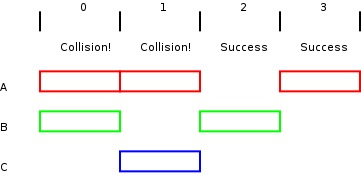
\includegraphics[scale=0.7]{slottedaloha.jpg}
\caption{Ejemplo de colisiones y éxitos en estructura ALOHA ranurado.\cite{ pagaloha2}.}
\label{fig:slottedaloha}
\end{center}
\end{figure}

\section{Replicator Dynamics para ALOHA}

Tal como se presenta en \cite{Mprincipal} se puede aplicar teoría de juegos evolutiva buscando...

\subsection{Descripción del juego}

Para escritura de símbolos matemáticos $A=  \left\lbrace T, S \right\rbrace$. \\
Si un agente $i$ realiza la transmisión de un paquete, este incurre en costo de trasmisión $\delta \geq 0$. La transmisión del paquete es exitosa y tienen una ganacia $V \gg \delta $ si todos los demás agentes que pueden interferir se mantienen en silencio, en caso contrario es una colisión y el costo correspondiente es $\Delta \geq 0$. Se puede dar que todos los agentes permanezcan en silencio (Stay quiet) lo cual genera un costo $\kappa$.\\ Finalmente se puden resumir y construir la función de pagos (Payoff function) $U_i : A^n \rightarrow  \mathbb{R} $ para cada usuario $i$ jugando su estrategia $a_i$ cuando se tiene una estructura fija y un numero $N$ de agentes involucrados\cite{Mprincipal}.

\begin{equation}
V=I*R
\end{equation}

\begin{equation}
U_i(a) = \left\lbrace
\begin{array}{lll}
V - \delta, &\textup{si}& a_i = T \textup{ y } a_j=S, \textup{   } \forall j\not= i\\
0 & \textup{si}& a_i =S \textup{ y } \lbrace j \in N | a_j=T\rbrace \geq 1\\
-\Delta - \delta & \textup{si}& a_i=T \textup{ y } \lbrace j \in N | a_j=T\rbrace \geq 2\\
-\kappa, &\textup{si}& a_j = S, \textup{     } \forall j \in N\\
\end{array}
\right.
\label{equ:payofffunction}
\end{equation}


\begin{eqnarray}
u_k(T,s) & = & (-\Delta-\delta)*(1-n_k)+(V-\delta)*n_k\label{eq:payoffT}\\
u_k(S,s) & = & -\kappa *n_k \label{eq:payoffS}
\end{eqnarray}

\begin{enumerate}
\item El nodo ....
\item El nodo ...
\item Masivamente...
\end{enumerate}




\begin{table}[]
\centering
\caption{Resultados Cantidad de transmisores ($s$) para distribución de Poisson}
\label{REsultadosJA}
\begin{tabular}{|c|c c c|}
\hline
\textbf{$\lambda$} & \textbf{Caso 1} & \textbf{Caso 2} & \textbf{Caso 3}         \\ \hline
        \hline
0.4 & 0.8742 & 0.7684 & 0.4287 \\
0.6 & 0.5828 & 0.5440 & 0.3524 \\
0.9 & 0.3886 & 0.3782 & 0.2749 \\
1.5 & 0.2331 & 0.2322 & 0.1887 \\
3.0 & 0.1166 & 0.1166 & 0.1048 \\
6.0 & 0.0583 & 0.0583 & 0.0553 \\
\hline
\end{tabular}
\end{table}


\begin{table*}
\centering
\caption{Titulo de la tabla que debido a su tamaño debe ocupar dos columnas del documento y romper el formato}
\begin{tabular}{c c}
\hline
\hline
&Tornillo micrométrico\\
&(mm)\\
\hline
&22,210\\
&22,230\\
&22,220\\
&22,220\\
&22,220 \\
&22,230 \\    
\multicolumn{2}{c}{Soy doble ocupo dos columnas}\\
\multirow{3}{*}{Soy triple} & 45\\
& 50\\
& 55\\
\hline
\hline
\end{tabular}
\end{table*}

\begin{table}
\centering
\caption{Titulo de la tabla que esta en una columna}
\begin{tabular}{c c}
\hline
\hline
&Tornillo micrométrico\\
&(mm)\\
\hline
&22,210\\
&22,230\\
&22,220\\
&22,220\\
&22,220 \\
&22,230 \\    
\multicolumn{2}{c}{Soy doble ocupo dos columnas}\\
\multirow{3}{*}{Soy triple} & 45\\
& 50\\
& 55\\
\hline
\hline
\end{tabular}
\end{table}



\section{Conclusiones}

Mediande la aplicación de replicadores dinámicos se logro observar y analizar el desempeño de un red basada en protocolo ALOHA la cual es la base para otras tecnologías de uso diario, logrando comprender el planteamiento basado en densidades de usuario conocidas y estimando costos de la comunicación.\\

Es importante resaltar que teniendo un avance en el análisis de desempeño de una red inalámbrica clásica, mediante la medición de la probabilidad de un envío exitoso por parte de un usuario, es necesario continuar el trabajo diseñando otras métricas necesarias en comunicaciones tales como eficiencia energética, uso del canal, tiempos de respuesta de las comunicaciones e incluso el análisis de interferencias y/o ruido.\\

Se concluye que el siguiente paso en la investigación de la temática referente al análisis de desempeño de redes inalámbricas de sensores es la implementación de diferentes algoritmos basados en replicators dynamics de mayor complejidad que sean capaces de proporcionar información adecuada sobre el valor esperado de desempeño, además de estudiar y comprender los algoritmos de enrutamiento necesarios para conexiones inalámbricas actuales.\\

\begin{thebibliography}{15}

\bibitem{M1} Abd, M.A.; Singh, B.K.; Al Rubeaai, S.F.; Tepe, K.E.; Benlamri, R., ``Game theoretic energy balanced (GTEB) routing protocol for wireless sensor networks,'' in \textit{Wireless Communications and Networking Conference (WCNC), 2014 IEEE }, vol., no., pp.2564-2569, 6-9 April 2014 doi: 10.1109/WCNC.2014.6952792

\bibitem{M1B} Abd, M.A.; Majed Al-Rubeaai, S.F.; Singh, B.K.; Tepe, K.E.; Benlamri, R., ``Extending Wireless Sensor Network Lifetime With Global Energy Balance,'' in \textit{Sensors Journal, IEEE }, vol.15, no.9, pp.5053-5063, Sept. 2015 doi: 10.1109/JSEN.2015.2432114

\bibitem{M5} Olariu, S.; Stojmenovic, I., ``Design Guidelines for Maximizing Lifetime and Avoiding Energy Holes in Sensor Networks with Uniform Distribution and Uniform Reporting,'' in \textit{INFOCOM 2006. 25th IEEE International Conference on Computer Communications. Proceedings }, vol., no., pp.1-12, April 2006 doi: 10.1109/INFOCOM.2006.296

\bibitem{M2} Shabani, H.; Ahmed, M.M.; Khan, S.; Hameed, S.A.; Habaebi, M.H., ``Smart Zigbee/IEEE 802.15.4 MAC for wireless sensor multi-hop mesh networks,'' in \textit{Power Engineering and Optimization Conference (PEOCO), 2013 IEEE 7th International} , vol., no., pp.282-287, 3-4 June 2013 doi: 10.1109/PEOCO.2013.6564558

\bibitem{M3} Qinghua Wang; Zhang, T., ``Characterizing the Traffic Load Distribution in Dense Sensor Networks,'' in \textit{New Technologies, Mobility and Security (NTMS), 2009 3rd International Conference on}, vol., no., pp.1-4, 20-23 Dec. 2009 doi: 10.1109/NTMS.2009.5384829

\bibitem{M4} Zhengyang Qu; Di Chen; Gaofei Sun; Xinbing Wang; Xiaohua Tian; Jing Liu, ``Efficient wireless sensor networks scheduling scheme: Game theoretic analysis and algorithm,'' in \textit{Communications (ICC), 2012 IEEE International Conference on }, vol., no., pp.356-360, 10-15 June 2012 doi: 10.1109/ICC.2012.6363753

\bibitem{Mprincipal} Hamidou Tembine; Eitan Altman; Rachid El-Azouzi and Yezekel Hayel, ``Evolutionary Games in Wireless Networks,'' in \textit{Systems, Man And Cybernetics - Part B: Cybernetics, 2010 IEEE Transactions on }, vol. 40, no. 3, pp. 634-646, June 2010 doi: 10.1109/TSMCB.2009.2034631

\bibitem{pagaloha1} Montañan, Rogelio ``4 Redes locales'', En línea [Diciembre 2 de 2015] \textit{http://www.uv.es/$\sim$montanan/redes/cap\_04.pdf}

\bibitem{pagaloha2} Hovemeyer, David, ``Networks Link Layer'', En línea [Diciembre 2 de 2015] \textit{}{http://faculty.ycp.edu/$\sim$ dhovemey/fall2005/cs375/lecture/11-16-2005.html}

\bibitem{Qua1} Wang, Yuanli; Liu Xianghui; Jianping Yin, ''Requirements of Quality of Service in Wirless Sensor Network'' in \textit{International Conference on Networking, Systems and Mobile Communications and Learning Technologies}. 2006.

\bibitem{GTWSN} Hai-Tan Shi, Wan-Liang Wang, Ngai-Ming Kwok and Sheng-Yong Chen, ''Game Theory for Wirless Sensor Networks: A Survey'' July 2006 doi: 10.3390/s120709055

\bibitem{PopGame} Hamidou Tembine, ''Population Games with Networking Applications''. Computer Science. Université d'Avignon, 2009. English.

\bibitem{PopProto} Dessart. Nathalie, Hunet. Philippe, Fouchal. Hacéne, Vidot. Nicolas ''Population Protocol Over Wireless Sensor Networks.'' Univ. des Antilles et de la Guyane, France. 2010. Conference: Local Computer Networks. doi 10.1109/LCN.2010.5735814.

\bibitem{STWSN2} Mao. Yuxin, Zhu. Ping, Wei. Guiyi '' A Game Theoretic Model for Wirless Sensor Networks with Hidden-Action Attacks''. in \textit{International Journal of Distributed Sensor Networks}. 2013. doi: 10.1155/2013/836056.

\end{thebibliography}

\end{document}
	
